\documentclass[twocolumn]{article}
\setlength{\columnsep}{30pt}
\usepackage[utf8]{inputenc}
\usepackage{url}
\usepackage{enumerate}
\usepackage{graphicx}
\usepackage[a4paper,hmargin=0.75in,vmargin=1in]{geometry}
\usepackage{color}
\usepackage{enumerate}
\usepackage{subfigure}
\usepackage{graphicx}
\usepackage{comment}
\newtheorem{thm}{Theorem}
\usepackage{algorithm}
\usepackage{algorithmic}
\usepackage{float}
\usepackage{multirow}
\usepackage{setspace}
\usepackage{bigints}
\usepackage{booktabs}
\usepackage{hyperref}
\usepackage{amsfonts}
\usepackage{listings} %插入代码
\usepackage{xcolor} %代码高亮
\lstset{basicstyle=\footnotesize, %\tiny or \small or \footnotesize etc.
        numbers=left, %设置行号位置
        numberstyle=\tiny, %设置行号大小
        keywordstyle=\color{blue}, %设置关键字颜色
        commentstyle=\color[cmyk]{1,0,1,0}, %设置注释颜色
        frame=single, %设置边框格式
        escapeinside=``, %逃逸字符(1左面的键),用于显示中文
        breaklines, %自动折行
        extendedchars=false, %解决代码跨页时,章节标题,页眉等汉字不显示的问题
        xleftmargin=0.5em,xrightmargin=0.5em, aboveskip=0.1em, %设置边距
        tabsize=2, %设置tab空格数
        showspaces=false %不显示空格
       }

%Use Chinese
\usepackage[UTF8]{ctex}

% command
\renewcommand{\algorithmicrequire}{\textbf{Input:}}
\renewcommand{\algorithmicensure}{\textbf{Output:}}

\title{图表示学习\\在Covid-19文献挖掘和知识发现中的应用}

\author{张世龙$^{1}$, 严晶$^{1}$,高飞宇$^{1}$}

\date{
\textsuperscript{1}华中农业大学信息学院}

%短文与长文只能从以下三个命题中挑选
%\begin{itemize}
%	\item 指定标题1: 《(第X章内容)在XX研究课题的研究概览》(Review)(三人中有2人以上非信息学院同学可以选此题)
%	\item 指定标题2: 《(第X章内容)在XX研究课题的应用》(代码使用+应用)
%	\item 指定标题3:《(第X章算法)代码开发及在XX研究课题的应用》(代码开发+应用)
%\end{itemize}
%其中“第X章算法”中的“X”章节编号以课程页面\url{https://hzaubionlp.com/course-bionlp-and-kd/}为依据。

\begin{document}
\maketitle

\begin{abstract}
新型冠状病毒肺炎(Covid-19)自从被发现以来,经历了地方性流行、流行、大流行的过程,并最终在全球范围内扩散蔓延。疫情爆发两年多以来,Covid-19已然成为最具影响力的话题之一,目前已有大量相关报道与文献。自然语言处理是一种大规模处理文献的有效手段,它研究能实现人与计算机之间用自然语言进行有效通信的各种理论和方法,而自然语言处理通过命名实体识别和实体关系识别,能够生成知识图谱以便于隐含信息挖掘。在该项目中,我们从PubTator获取文献实体标注信息开始,到知识图谱的生成,和图表示学习与信息挖掘,期望推测出化合物与Covid-19基因相关的结论。\par
{\bf Codes availability:} \url{https://github.com/zhang-shilong/BioNLP-course}。\par
{\bf 关键词: NLP,Covid-19,图表示学习,知识发现}
\end{abstract}

\maketitle

\section{概况}
\subsection{选题说明(本章节作者:高飞宇)}
自然语言处理(Natural Language Processing, NLP)是计算机科学领域与人工智能领域中的一个重要方向,它研究能实现人与计算机之间用自然语言进行有效通信的各种理论和方法。选修该课程目的在于学习通过对文献中的文本数据进行挖掘地技能,更高效地获得知识发现,优化研究方法。\par
根据世界卫生组织最新实时统计数据,截至北京时间2022年4月7日6时30分左右,全球累计确诊新冠肺炎病例494928850例,累计死亡病例6186342例,对世界各国均产生了不可估量的影响,目前相关文献数目庞大,但我们对其了解还不够深入。因此选取该课题旨在高效挖掘文献摘要中的实体信息并进行知识发现,为Covid-19相关研究如致病机理、药物靶点、疫苗研发等,提供一定的参考意义。\par
本项目期望从文献中获取“主语-谓语-宾语”三元组构建知识图谱,利用图表学习算法挖掘出化合物与Covid-19基因的关系,如新冠病毒某个基因的表达受到某个化合物的激活作用等。\par

\subsection{该算法基本原理(本章节作者:张世龙)}
我们计划从Covid-19相关的科学文献中识别命名实体,再抽取“主语-谓词-宾语”的三元组信息,将自然语言转换为知识图谱,再使用链接预测算法挖掘基因和化合物之间的隐含信息。\par
知识图谱是一种便于进行推理的图结构。面向知识图谱的推理主要围绕关系的推理展开,即基于图谱中已有的事实或关系推断出未知的事实或关系,一般着重考察实体、关系和图谱结构三个方面的特征信息。具体来说,知识图谱推理主要能够辅助推理出新的事实、新的关系、新的公理以及新的规则等。\par
链接预测(Link Prediction)是图表示学习的应用方向之一,其方法是将知识图谱中实体和关系的内容映射到连续向量空间中,对知识图谱中的关系进行预测。链接预测算法在生物医学领域可以用于发现可能发生相互作用的实体,在我们的项目中用于发现可能有关联的“基因-化合物”,即寻找哪些化合物对基因可能产生作用,进而为Covid-19治疗挖掘可能有效的药物。\par
我们定义一个有标签的有向图,即多个不同标记的边可以连接相同结点对的图,表示为知识图谱$KG=(\mathcal{E}, \mathcal{R}, \mathcal{G})$\cite{link_prediction}:
\begin{itemize}
	\item $\mathcal{E}$:表示结点的集合,每个结点对应一个实体;
	\item $\mathcal{R}$:表示关系的集合;
	\item $\mathcal{G} \subseteq \mathcal{E} \times \mathcal{R} \times \mathcal{E}$:边集,表示每对关联实体及其关系,每个元素表示为一个三元组$\langle h, r, t\rangle$,其中$h$是头实体,$r$是关系,$t$是尾实体。
\end{itemize}\par
链接预测的任务是利用知识图谱中的现有事实来推断缺失的关系,相当于预测三元组$\langle h, r, t\rangle$的某个缺失部分。链接预测的数据集通常是由真实世界的知识图谱采样得到的,这些采样得到的小型知识图谱也分别具有自身的结点集$\mathcal{E}$,关系集$\mathcal{R}$和边集$\mathcal{G}$。为方便研究,$\mathcal{G}$被分割为训练集$\mathcal{G}_{train}$和测试集$\mathcal{G}_{test}$。\par

\subsubsection{损失函数}
在训练中,嵌入通常是随机初始化的,然后使用梯度下降的反向传播等算法进行优化。模型还可以学习不特定于任何神经网络元素的其他共享参数(例如,神经层的权重)。链接预测算法可以作为一种有监督的学习任务,将网络中存在的边都视为正样本,不存在的连边都当作负样本,训练过程最终旨在为嵌入和共享参数找到最大化正样本的合理性同时最小化负样本的合理性的值。在训练集中的正样本表示为$\mathcal{G}_{train}$,负样本表示为$\mathcal{G}_{train}^{corr}$。损失函数需要综合考虑$\mathcal{G}_{train}$和$\mathcal{G}_{train}^{corr}$中所有关系的分数。\par
负对数似然(Negative Log-Likelihood,NLL)是一种标准的损失函数,且在链接预测领域广泛流行:
$$\mathcal{L}=\sum_{\langle h, r, t\rangle \in \mathcal{G}_{\text {train }} \cup \mathcal{G}_{\text {train }}^{c o r r}} \log \left(1+e^{-y_{h r t} \phi(\boldsymbol{h}, \boldsymbol{r}, t)}\right)$$
其中当$\langle h, r, t\rangle \in \mathcal{G}_{train}$时,$y_{hrt}=+1$;当$\langle h, r, t\rangle \in \mathcal{G}_{train}^{corr}$时,$y_{hrt}=-1$。在这个公式中,得分较高的阳性样本会降低$\mathcal{L}$,而得分较高的阴性样本会增加$\mathcal{L}$。因此,最小化$\mathcal{L}$意味着最大化训练集正样本的分数,同时最小化训练集负样本的分数。\par

\subsubsection{链接预测方法}
根据不同方法的损失函数和空间复杂度,链接预测方法可以分为3大类,分别是张量分解模型、几何模型和深度学习模型\cite{link_prediction}。开源Python库PyG(PyTorch Geometric)是一个基于PyTorch的图神经网络框架,鉴于其易用性和可扩展性,我们选择PyG进行链接预测算法深度学习模型的实现。\par
深度学习模型使用深度神经网络来执行链接预测任务。在链接预测领域,知识图谱嵌入通常与层的权重和偏差一起学习,这些共享参数使这些模型更具表现力,但训练时间可能更长,更容易过度拟合。根据他们使用的神经网络结构,可以为分为三种:(i)卷积神经网络,(ii)胶囊神经网络,以及(iii)递归神经网络(RNN)\cite{link_prediction}。\par
在以上三种网络模型中,卷积神经网络是用于链接预测实例最多的神经网络模型。这些模型依靠卷积层对输入数据(例如,知识图谱训练集关系中的嵌入)进行卷积,并应用低维滤波器$\omega$。结果是一个特征图,然后通常将其传递到其他网络层,以计算关系分数。我们的项目中可能会使用卷积神经网络作为深度学习模型完成链接预测任务。\par
胶囊神经网络由一组称为胶囊的神经元组成,胶囊对输入的特定特征进行编码,例如图像中特定物体的存在。Capsnet可以像卷积网络那样识别这些特征,而不会丢失空间信息。每个胶囊将其输出发送到更高阶的胶囊,连接由动态路由过程决定。\par
递归神经网络使用一个或多个重复层来分析从训练集中提取的整个路径(事实序列),而不是单独处理单个事实。循环跳过网络(RSN)是专门为链接预测算法设计的一种RNN。由于实体和关系的变化,基本RNN可能不适用于链接预测,因此作者提出了一个新的层来积极考虑这一方面。由此产生的RSN模型通过有偏随机游动学习从训练集中提取的整个路径,并使用一种特别优化的基于类型的NCE损失。\par
使用图神经网络进行链接预测主要分为以下5步:\par
\begin{enumerate}
	\item 导入图数据;
	\item 分割数据集(划分训练集、验证集和测试集);
	\item 标注正样本、采样负样本;
	\item 训练神经网络;
	\item 测试模型效果。
\end{enumerate}\par

\subsubsection{评估指标}
在知识表示学习领域,普遍采用链接预测实验对模型的效果进行评估。在链接预测预测任务中,我们需要将测试集中的每个三元组$\langle h, r, t\rangle$中的头实体($h$)或尾实体($t$)依次替换为字典里的所有实体。这些替换后的三元组被称为 corrupted triplets,即损坏的三元组。然后我们通过模型的评分函数对这些 corrupted triplets 进行评分并降序排列。显然,由正确的实体构成的那个三元组的排名越靠前,说明模型对实体的预测能力就越强。\par
对于链接预测任务,主要有 Mean Rank 和 $Hits@K$ 这两项评测指标。\par
在完成评分排名后,找到正确的三元组,整个测试集的所有正确三元组的平均排名就作为 Mean Rank(MR):
$$MR=\frac{1}{|Q|} \sum_{q \in Q} q$$
由于MR对异常值极其敏感,因此逐渐被Mean Reciprocal Rank (MRR)替代:
$$MRR=\frac{1}{|Q|} \sum_{q \in Q} \frac{1}{q}$$
而 $Hits@K$($H@K$) 则指的是正确三元组排在前$K$名的概率,即排在前$K$的个数与总个数的比值:
$$H @ K=\frac{|\{q \in Q: q \leq K\}|}{|Q|}$$


\section{研究方法}

\subsection{PubTator实体标注(本章节作者:严晶)\label{data_access}}
文献知识发现的实现首先需要从PubMed获取Covid-19相关文献的PMID。虽然可以直接从官网匹配筛选条件进行下载,但考虑网站下载数量以及速度的限制可能会产生的大量人力物力成本,因此选择了使用NCBI提供的Entrez获取PMID。\par
Entrez检索库是一个检索系统,可以快速高效地实现从PubMed上下载满足条件的文献PMID、标题、摘要等。通过设置文献筛选的限制条件,包括词汇匹配以及时间限制等,Entrez.esearch可以实现有关文献的检索。\par
我们使用Python语言的Biopython库,以“Covid-19”为检索条目,要求出版时间为2021年7月1日至2022年3月1日,从Entrez获取PMID共81290条。\par
PubTator作为一个基于web的生物类自动化文本挖掘工具,易于操作,能够实现特定于实体的语义搜索并为计算机辅助生物鉴定提供预注释,自动对实体进行识别标注。Pubtator可以识别并标注的实体类型有基因、疾病、化合物、突变、物种和细胞系,能够为生物医学文献的注释提供极大帮助。\par
我们使用Python语言调用了PubTator的API,获取PMID对应文献的标题、摘要和实体标注结果。由于PubTator要求每秒请求次数不能超过3次,所以该步骤耗时极长,我们将其部署在服务器上运行。最终获取PubTator标注994561条,其中基因标注56091条,化合物标注69362条。\par

\subsection{实体频次统计(本章节作者:高飞宇)\label{chap:entity_count}}

\begin{table*}[ht!]
	\centering
	\caption{Covid-19化合物标注频次统计。本表自绘,数据来源:统计Pubtator标注的实体}
	\begin{tabular}{cccc}
		\hline
		化合物类型 & 标识符 & 频次 & 描述\\
		\hline
		oxygen & MESH:D010100 & 2759 & 氧气\\
		remdesivir & MESH:C000606551 & 2008 & 瑞德西韦\\
		alcohol & MESH:D000438 & 1779 & 酒精\\
		omicron & - & 1401 & 奥密克戎\\
		tocilizumab & MESH:C502936 & 1323 & 白介素-6(IL-6)受体抑制剂\\
		dexamethasone & MESH:D003907 & 874 & 地塞米松\\
		\hline
	\end{tabular}
	\label{tab:mutation}
\end{table*}

\begin{figure*}[ht!]
	\centering
	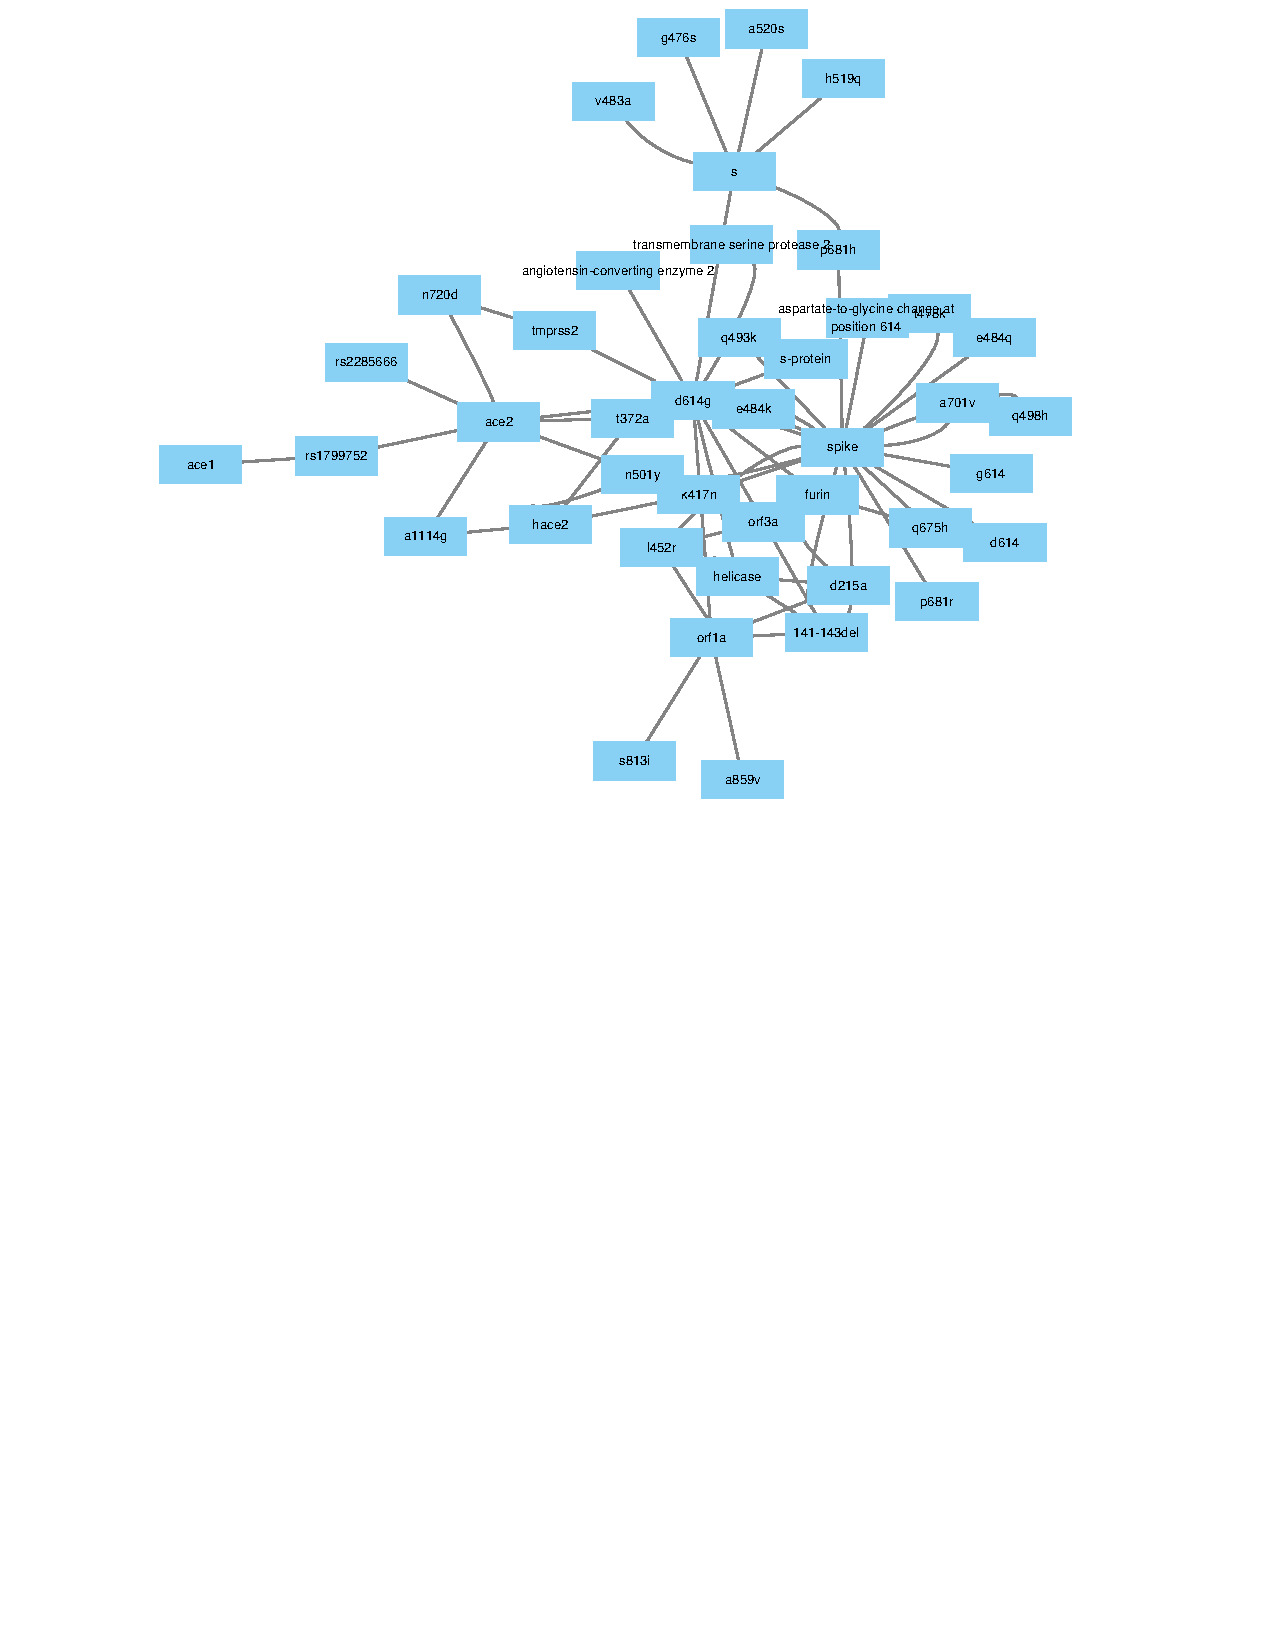
\includegraphics{figure/gene_mutation_visualization.pdf}
	\caption{基因和Covid-19突变类型关联可视化。本图自绘,绘图工具:Cytoscape}
	\label{fig:cosentence}
\end{figure*}

\begin{table*}[ht!]
	\centering
	\caption{基因和化合物关系。本表自绘,数据来源:统计已标注实体的共句情况}
	\begin{tabular}{cccc}
		\hline
		基因 & 化合物 & 频次 & 描述\\
		\hline
		Spike & Omicron & 72 & Omicron与Spike的突变有关\\
		ACE2 & Omicron & 44 & Omicron突变改变了与ACE2的结合性\\
		TMPRSS2 & serine & 40 & TMPRSS2与丝氨酸有关\\
		C-reactive protein & oxygen & 39 & 该蛋白与氧气有关,可能是无效关系\\
		PF4 & heparin & 34 & PF4与heparin有关\\
		ACE2 & creatinine & 24 & ACE2与creatinine有关\\
		\hline
	\end{tabular}
	\label{tab:gene_mutation}
\end{table*}

现在,我们已经得到了PubTator对Covid-19相关文献的实体标注信息,可以对实体频次做进一步统计分析。\par
为了推测出对Covid-19较为有效的治疗方法,我们对所有化合物标签进行统计,可以得到在这些文献样本中被讨论最多的与Covid-19相关的化合物,如表\ref{tab:mutation}所示。除此之外,我们还进行了基因和Covid-19突变类型的可视化,如图\ref{chap:cosentence}所示。\par
这些化合物可能对Covid-19的治疗有一定帮助,因此对这些化合物进行分析,对数据进行筛选后,发现出现次数较多的化合物可分为两类,一类是Covid-19相关基因的靶标化合物,另一类是抗RNA病毒感染的化合物。Covid-19为正链RNA病毒,也从一定程度上证明这些化合物可能与Covid-19的治疗相关。\par
Remdesivir是一种核苷酸模拟前药,具有广泛的抗病毒活性,在治疗恒河猴SARS-CoV-2感染模型中发现,Remdesivir治疗的动物的肺病毒载量较低,对肺的损害也有所减少\cite{PPR:PPR151409},这对于Covid-19的临床治疗有极大的参考意义。酒精(alcohol)一直以来也被认为是肺部病理生理学的一个促成因素,酒精肺是COVID-19易感性和严重程度的负面后果的极有可能并发症\cite{BAILEY202111},所以在Covid-19大流行期间,alcohol的合理使用也是值得讨论的问题。\par
实体频次统计过程中,发现的出现次数较多的化合物可能对Covid-19的治疗有显著作用,通过研究这些化合物或可发现Covid-19治疗的新方法。\par
实体频次统计过程中发现,同义实体可能具有多个名称,例如Spike、S protein和S都表示新冠病毒的刺突蛋白,coronavirus disease 2019、Covid-19和covid都表示新型冠状病毒肺炎。这些异名同义实体出现次数较多,可能影响后续分析结果,在下一阶段可以通过列出异名同义实体表或选择更加智能的命名实体识别算法来解决这个问题。\par

\subsection{共句分析(本章节作者:严晶)\label{chap:cosentence}}
针对PubTator标注的实体,我们认为当两个实体倾向于出现在同一语句中时可以说明它们之间存在着某种潜在关联。通过Python编写的程序,我们对之前步骤中处理过的基因实体数据、化合物实体数据,以及摘要数据进行了读取,并尝试了通过判断基因与化合物是否存在于同一语句中,确定其中的潜在关联,并格式化输出了Covid-19相关的基因与化合物之间的互作关联文件,以便于后期Cytoscape的读取与可视化,部分结果如表所示。\par
当两个实体出现在基因-化合物关系结果中时,有以下四种可能情况:
\begin{itemize}
	\item 新冠病毒的某个基因受某种小分子化合物或药物作用,而改变其传播性或生理活性;
	\item 新冠病毒受体的基因受某种小分子化合物或药物作用,而改变受体与新冠病毒的结合性;
	\item 无明显关联的基因和化合物,该情况在共句分析中同样会出现。
\end{itemize}

我们期望通过实体的共句分析,确定基因与对应化合物之间的互作关联,进而为药物靶点筛选、Covid-19病毒入侵机制的研究以及Covid-19的预防与监控提供一定程度的参考。对此,我们针对基因-化合物的互作关系在Cytoscape进行可视化,绘制了关联网络,以直观展示它们的关联信息。图中显示了Omicron与Spike有高度的关联性,而与Tip、CD20和RBM等基因关联度较低。以为Omicron例,Omicron与Spike相关联,该刺突蛋白突变可以抑制机体产生免疫应答,对病毒起到保护作用\cite{spike},这进一步说明了Omicron化合物的存在可能与刺突蛋白的表达存在着一定的关联关系。除此之外,creatinine与C-reactive protein呈现强关联,该基因与化合物呈现的高度相关性在众多文献中均有证明,因此也从一定程度上说明了本实验的可靠性。同时,ACE2(血管紧张素转化酶2)基因已被证明是新冠病毒刺突蛋白感染细胞的主要受体,serine、aldosterone等化合物与ACE2基因的高度关联性也为我们从新冠病毒有关化合物与基因的相互作用入手探索新冠病毒变体感染力改变的关键因素提供了一定的参考。\par
共句分析只能表明某两个实体之间存在关联,但不能确定关系的类别。下面我们将抽取关系生成“主语-谓词-宾语”三元组,生成知识图谱来助力隐含信息挖掘。\par

\subsection{三元组抽取(本章节作者:张世龙)\label{chap:triple}}

至此为止,我们已经获得了哪些实体倾向于出现在同一语句中,即已经获取了“主语-谓词-宾语”三元组中的主语和宾语,而谓词包含了两个实体之间的关系,对于知识推理非常重要。本章节中,我们主要研究完整三元组的抽取方法。\par
spaCy是自然语言处理方面的一个Python库,它包含多种已训练的模型,以此来执行执行一些与NLP相关的任务,例如词性标记、命名实体识别和依存关系解析。spaCy以其高功能性和高灵活度著称,开发者自行训练的模型或开发的插件等都可以方便地接入spaCy,这极大地提高了spaCy在生物医学文本上的适用性。\par

\subsubsection{模型选用}
在自然语言处理研究中,使用领域专业文本训练的模型准确率会得到极大地提高。ScispaCy便是一个以spaCy为基础开发的Python库,其中包含了用于处理生物医学、科学或临床文本的spaCy模型。我们分别使用了spaCy模型en\_core\_web\_sm和ScispaCy模型en\_core\_sci\_sm对同一文本的命名实体识别进行测试,查看两个模型的实体识别准确度。\par
测试文本:\\
SARS CoV-2 is the causative agent of coronavirus disease-19 (Covid-19).\par
spaCy实体识别结果:\\
SARS \fbox{CoV-2 ORG} is the causative agent of coronavirus \fbox{disease-19 PERSON} (Covid-19).\par
ScispaCy实体识别结果(识别类型全部为ENTITY):\\
\fbox{SARS} \fbox{CoV-2} is the \fbox{causative agent} of \fbox{coronavirus disease-19}  (\fbox{Covid-19}).\par
spaCy将CoV-2识别为组织,将disease-19识别为人名,且都没有识别出完整的词汇。ScispaCy实体识别基本正确,仅未识别出SARS和CoV-2应为一个实体,这可能是SARS(非典型性肺炎)已经是一种病的名字导致的。\par
两个模型得到的句法依存树等结果也不相同,且ScispaCy的en\_core\_sci\_sm模型在生物医学文本上有明显优势,后续将使用ScispaCy的模型继续分析。\par

\begin{figure*}[ht!]
	\centering
	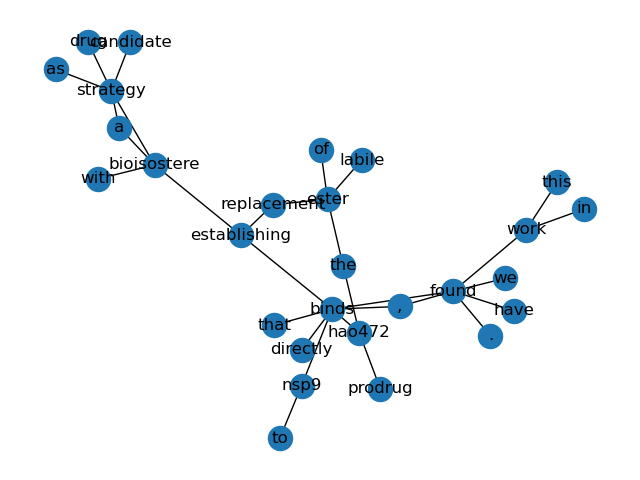
\includegraphics[width=\textwidth]{figure/sdp.png}
	\caption{句法依存树。本图自绘,绘图工具:matplotlib}
	\label{fig:sdp}
\end{figure*}

\subsubsection{句法依存分析\label{chap:dep}}
句法依存树是句法分析的重要方法,它是用来提取句子中所有从属词(dependent)的支配词(head)以及二者依存关系(dependencerelation)的方法。spaCy正提供了这种语法依存树的分析方法,且和NetworkX结合,可以简单地实现可视化和最短路径搜索。而对于如何从句法依存树中获取两个实体之间的关系,即三元组中的谓词,我们产生了不少争论。\par
我们首先想到的是使用句法依存树的根作为谓词,必要时还可以添加根的修饰词,以精确确定谓词。但是,论文摘要中的句子多是长难句,且重要内容总是出现在从句中。例如下面这个句子是论文摘要中的常见结构,通常以“我们发现了”、“我们认为”等开头,而重要内容位于宾语从句中(PubTator识别出的实体用矩形标识,句法依存树见图\ref{fig:sdp})。从下面这个句子中获得的根是“found”,显然不是实体之间的关系,因此直接从句法依存树获取根和根的修饰词作为关系,是不合理的。\\
In this work, we have found that the prodrug \fbox{HAO472} directly binds to \fbox{Nsp9}, establishing replacement of the labile \fbox{ester} with a bioisostere as a candidate drug strategy.\cite{hao472}\par
既然句法依存树的根不可靠,我们计划从最短依存路径(Shortest dependency path,SDP)中抽取实体关系。SDP描述了两个实体之间的最短依存关系,其经过的路径可能就是我们要找的实体关系。令人欣慰的是,SDP在\cite{hao472}中获得了不错的结果,它得到了“HAO472 binds Nsp9”的正确结果,如果我们对谓词的修饰词加以限制性的选用,甚至可以得到“HAO472 directly binds Nsp9”这样更优秀的结果(详见\ref{chap:modifier}节)。而对于搜索多个候选实体之间的关系时,我们再次陷入了困境,如HAO472或Nsp9与ester之间有两条SDP可供选择:\par
\begin{itemize}
	\item \textbf{HAO472} the \textbf{ester}
	\item \textbf{Nsp9} binds establishing replacement \textbf{ester}
\end{itemize}\par
显然,后者取得了更优质的结果,尽管语句并不通顺。至于为何得到了前一个结果,我们会在\ref{chap:dep_eva}节讨论。\par

\subsubsection{多候选实体的SDP搜索}
我们可以观察到,HAO472与Nsp9结合,在句法依存树上HAO472和Nsp9分别作为binds的名词性主语(nsubj)和nmod(名词修饰词)。如果将HAO472和Nsp9调换位置,让Nsp9作为名词性主语,HAO472作为名词修饰词,该语句同样是成立的,也就是说,如果只从HAO472出发,则忽略了Nsp9到ester的关系。因此,我们做出一个大胆猜测,当HAO472和Nsp9同属于binds的近似依存关系时,SDP的搜索可以从binds开始,到ester结束。泛化地讲,当两个同类型实体同属于某个相邻结点的近似依存关系时,SDP从这两个相邻实体的相邻结点开始,到另一类型的候选实体结束。关于如何确定依存关系近似,我们认为当这两个同类型实体,其中一个属于nsubj(名词性主语)或nsubjpass(被动名词性主语),而另一个属于nmod(名词修饰词)时,称这两个实体依存关系近似,这是由于识别出的实体都是名词性的,且一个作为主语,另一个作为修饰词。\par
多候选实体的SDP搜索算法如算法\ref{alg:multi_sdp}所示。当$e$存在多个时,依次遍历这些实体并执行算法\ref{alg:multi_sdp}即可。在\cite{hao472}的例句中,$S_C$指HAO472和Nsp9,它们都被Gene标签标注,$e$指ester,被Chemical标签标注。算法中寻找到的$h$指binds,返回结果$P$为“binds establishing replacement ester”,加上Gene实体即构成了完整的最短依存路径:\par
\begin{itemize}
	\item \textbf{HAO472} binds establishing replacement \textbf{ester}
	\item \textbf{Nsp9} binds establishing replacement \textbf{ester}
\end{itemize}\par
在此做法的情况下,完美避开了\ref{chap:dep}节所述的“HAO472 the ester”这样的错误SDP。\par

\begin{algorithm}[htb]
	\caption{多候选实体的SDP搜索算法}
	\label{alg:multi_sdp}
	\begin{algorithmic}[1]
		\REQUIRE
		同类型候选实体的集合$S_C$;
		另一类型的候选实体$e$;
		语句对应的句法依存树$G$;
		\ENSURE
		从$S_C$到$E$的最短依存路径$P$;
		\FOR{\textbf{each} $node \in G$}
		\IF{$S_C$中的所有实体都作为$node$的支配词,且依存关系近似}
		\STATE $h \gets node$
		\ENDIF
		\ENDFOR
		\IF{$h$ exists}
		\STATE $P \gets$ shortest\_path($G$, source=$h$, target=$e$) 
		\ENDIF
		\RETURN $P$
	\end{algorithmic} 
\end{algorithm}

\subsubsection{修饰词限制性选用\label{chap:modifier}}
现在,我们已经对一对一(两个候选实体)和一对多(多个候选实体)的句法依存分析和SDP搜索方法展开了讨论,能够得到不错的结果。\par
然而,生物医学文本用词考究,副词等修饰词也能对语义产生重大影响,我们的关系提取方法不能忽略这些修饰词。例如,directly bind和indirectly bind都描述了两个实体具有bind互作关系,但直接结合表示两个实体有相互结合的作用位点,间接结合表示两个实体有相互作用,但并不存在相互结合的作用位点。因此,SDP搜索过程中需要对修饰词进行选用,将合适依存关系的修饰词纳入SDP路径中。\par
我们认为,SDP搜索过程中,如果遇到从属词存在nsubj(名词性主语)、nmod(名词修饰词)、amod(形容词修饰词)、advmod(副词修饰词)依存关系的支配词时,将该支配词加入路径。我们规定,额外的支配词加入路径时,需要根据与从属词的依存关系决定加入位置:名词性主语和名词修饰词加到从属词后,形容词修饰词和副词修饰词加到从属词前,以更符合自然语言的语序。\par
通过以上一系列精细地关系抽取步骤后,\cite{hao472}中的例句中可以提取到3条精确的关系(修饰词用斜体表示):\par
\begin{itemize}
	\item \textbf{HAO472} \textit{directly} binds \textbf{Nsp9}
	\item \textbf{HAO472} \textit{directly} binds \textit{Nsp9} establishing \textit{bioisostere} replacement \textit{labile} \textbf{ester}
	\item \textbf{Nsp9} \textit{directly} binds \textit{HAO472} establishing \textit{bioisostere} replacement \textit{labile} \textbf{ester}
\end{itemize}\par

\subsubsection{效果评价\label{chap:dep_eva}}
在\ref{chap:dep}节,我们得到了“\textbf{HAO472} the \textbf{ester}”这样一个匪夷所思的结果,然而HAO472和ester不可能在语法依存树上直接与the相连,这究竟是什么原因导致的呢?老师提供的将spaCy句法依存树转换为NetworkX网络的代码是不严谨的,将每个token作为结点的名称,而NetworkX会将名称相同的结点视为同一个结点并进行合并。例句中恰好有两个the,它们将HAO472和ester巧合地连接在一起。\par
将spaCy句法依存树转换为NetworkX网络的正确途径,应该是借助spaCy库Token类的orth属性,它是spaCy为文本逐词分配的唯一ID。首先创建一个从orth到文本词语的映射字典,便于后期通过orth检索原始文本词语;再使用orth作为NetworkX网络的结点名称,构建句法依存树;最后,由于orth阅读不便,句法依存树可视化时应使用原始文本词语作为显示的结点名称。\par
本文提出的多候选实体SDP搜索算法和修饰词选用都是基于我们对于句法的浅薄理解,可能忽略了很多句法上的问题,例如修饰词选用时其他依存关系对应的支配词也应该被选用等,能够解决的问题有限。\par
到此为止,我们已经在三元组抽取方面讨论了模型选用、句法依存分析、多候选实体的SDP搜索和修饰词限制性选用等问题,我们尽可能地让三元组包含最多且最精确的信息。概括地说,我们首先根据NER的效果选择合适的模型,发现使用生物医学文本训练的ScispaCy效果更优;其次构建句法依存树,发现SDP得到的部分结果尚可,而对于多候选实体时只有一对实体能得到正确结果;然后对多候选实体的SDP搜索提出优化算法,使得多个候选实体都能得到正确的结果;最后精益求精,在SDP搜索路径中加入修饰词,得到了更加精确的实体关系。\par

\subsection{图表示学习(本章节作者:张世龙)\label{chap:embedding}}
我们已经得到了从自然语言文本中一步步抽取出的“主语-谓词-宾语”三元组信息,每个三元组实际上描述了从“主语”到“宾语”、关系为“谓词”的边,因而这些三元组共同构成了一张知识图谱。PyG(PyTorch Geometric)是一个基于PyTorch构建的库,可以方便地编写和训练图神经网络(GNN)。下面我们将使用PyG进行知识图谱的链接预测算法,尝试挖掘出潜在的“基因-化合物”信息。\par
在该步骤中,我们计划:\par
\begin{itemize}
	\item 首先使用Python库DeepSNAP将NetworkX网络转换为PyTorch能够识别的数据格式,这个包提供了NetworkX到PyG的接口;
	\item 我们计划使用有监督的链接预测算法,即将其视为二分类任务,将网络中存在的边都视为正样本,将网络中不存在的边视为负样本;训练集和测试集中都包含正样本和负样本,目的是在训练集上训练出一个模型能够准确分类这两种边,然后再在测试集上验证效果;
	\item 由于我们得到的知识图谱是比较稀疏的,在有监督学习中就意味着负样本远大于正样本,类别极其不平衡。我们可能需要采取负采样策略,每次训练的时候随机抽取与正样本等比例的负样本,避免类别不平衡;
	\item 有些化合物被研究较少,所以在知识图谱中的连接度较低,但这并不说明它是不重要的,每个不被重视的化合物也有可能就是我们要寻找的Covid-19治疗药物,所以我们未来对这一问题也会展开讨论;
	\item PyG还提供了一些论文中所使用的模型,我们可以使用他人已训练好的模型,来进行链接预测算法。
\end{itemize}\par
本部分将在下次论文提交前实现。


\section{后记}

\subsection{课程论文构思和撰写过程(本章节作者:高飞宇)}
本次课程项目主要是对海量Covid-19相关文献进行挖掘,并对在其中获得与化合物、基因相关的实体进行标注、统计、分析和抽取,发现潜在的、隐含的知识。我们首先使用NCBI提供的Entrez获取到与Covid-19相关文献的81290条PMID,调用PubTator的API获取相关文献的标题、摘要和实体标注结果。对相关实体进行频次统计,得到出现次数最多的化合物,认为这些化合物对Covid-19的治疗有显著关系,并可以为其治疗提供新思路。当两个实体倾向于出现在同一语句中时,可以从一定程度上说明其存在潜在关系,因此通过分析基因与化合物的互作关联,可以为药物靶点筛选、Covid-19病毒入侵机制的研究以及Covid-19的预防与监控提供一定程度的参考。但共句分析只能说明两个实体字间存在关联,并不能确定其关系类别,因此我们进一步对其进行了三元组抽取,这也是本次课程项目的核心步骤。我们从文献中获取“主语-谓语-宾语”三元组构建知识图谱,进行句法依存分析、多候选实体的SDP搜索以及修饰词限制性选用,以此得到最终实体之间的精确关系。同时本次的项目也能够解决人工阅读文献费时费力且效率不高有信息遗漏等问题,挖掘出大量信息,为Covid-19相关药物以及意面研发等科学研究提供一定的参考意义。\par

\subsection{所参考主要资源(本章节作者:张世龙)}
目前,我们参考的主要资源主要有:
\begin{itemize}
	\item 夏老师提供的《生物文本挖掘与知识发现概论》Course Note,我们主要参考了“依存树和最短依存距离计算的方法”;
	\item 链接预测算法的介绍和基本原理,我们主要参考了\cite{link_prediction}。
\end{itemize}

\subsection{论文选题与课程内容的对应关系(本章节作者:严晶)}
考虑到论文选题Covid-19的文献的数量级,我们在课堂老师介绍的手动搜索并复制粘贴PMID进行实体数据下载的基础上进行了改进,选择了使用Python的BioPython库中的Entrez检索库,通过设置文献筛选的限制条件,包括词汇匹配以及时间限制等,快速高效地从PubMed上获取了满足条件的文献PMID。\par
实体获取参考了课程所讲授的内容,即获取文献PMID后,编写脚本利用PubTator工具获取对应文献的标题和摘要信息,再针对获取的信息进行分析处理,提取有关实体信息,不同之处在于我们并未直接使用课程老师介绍的脚本,而是在完全理解课堂的Shell脚本的原理之后自主编写了Python脚本。\par
除了课堂讲授的PubTator实体抽取,我们还补充了实体词频分析、共句分析、三元组抽取等分析方法去实现Covid-19文献的知识挖掘。其中,句法依存树的构建和SDP的方法参考了课程讲义的第9章“Advanced NLP Topic in Dependency Tree and Shortest Dependency Path”。\par
在本项目中,所有代码内容均为在充分理解和参透课堂内容的基础上自主编写完成。\par

\subsection{代码撰写的构思和体会(本章节作者:张世龙)}
本项目中涉及的论文撰写工作主要有:调用Entrez API获取PMID,调用PubTator API获取标题和摘要的注释信息,实体频次统计和共句统计,实体关系抽取(SDP的实现和扩展),基于PyG的链接预测算法。\par
代码撰写的难点主要在于对陌生开源库不熟悉,需要不断地查询API文档,而有些API文档不便于理解,还需要在网上查询他人对API的使用方法。\par
实体关系抽取一节,夏老师提供了使用spaCy分析语句并构建句法依存树的方法,我们使用了这些代码。在使用spaCy的自带模型en\_core\_web\_sm时,我们发现它对生物医学文本命名实体识别和句法分析的效果很差,甚至连新冠病毒肺炎也无法识别。随后我们发现了ScispaCy库的en\_core\_sci\_sm模型,它是基于生物医学文本训练的,能够胜任我们Covid-19文献挖掘的任务。夏老师的讲义给了我们很大的灵感,使用SDP来发现两个实体之间的关系的确是一种好办法。但我们发现传统的SDP方法在涉及多个实体时只能识别正确一部分关系,且识别出的关系表意不明,因此我们提出了多候选实体的SDP搜索算法,改善了实体数量较多时的关系识别。除此之外,我们还为关系加入了名词、形容词和副词词性的修饰词,期望获得更加准确的实体关系。\par
链接预测算法一节,PyG是一个基于PyTorch构建的库,专业于图神经网络,为我们提供了极大的方便。该部分代码将在下次论文提交前实现。

\subsection{人员分工(本章节作者:张世龙)}
论文构思:共同讨论。\par
代码撰写:张世龙。\par
论文撰写:张世龙,严晶,高飞宇。\par

\subsection{本课程论文的主要优点和缺点(本章节作者:严晶)}
优点:\par
\begin{itemize}
	\item 聚焦于Covid-19有关基因与化合物的互作关联,从一个新的角度为新冠病毒的治疗与预防提供了一定的参考方向;
	\item 通过Python脚本的编写解决了PubMed网站上直接下载获取PMID上限10000的局限性,且大大降低了获取PMID所需的时间成本;
	\item 基因-化合物的互作关联知识图谱的绘制直观地展示了基因与化合物之间的关联关系,对于有关基因和化合物的研究提供了便利;
	\item 通过有效的实体关系识别算法识别正相关或负相关关系,生成了“主语-谓词-宾语”三元组,确定了实体之间存在的关系类别。
\end{itemize}\par
缺点:\par
\begin{itemize}
	\item 命名实体识别中存在着异名同义的现象,但在本项目中对该问题有所忽视,因此未能及时解决其带来的有关问题;
	\item PubTator相较于BERT+CRF等神经网络训练出来的模型效果稍有欠缺,但由于时间原因,我们在本次项目中舍弃了效果更佳的方案,而采用操作更为方便的PubTator;
	\item 对于基因与化合物的互作分析研究仅涉及文献单个层面,其可靠性仍然有待考量。
\end{itemize}\par

\subsection{假设多出30个工作日,这个课程论文的撰写改进思路和周工作计划(本章节作者:严晶)}
若时间充足,后续课程论文撰写改进将从技术层面以及论文层面两个方向进行改进:\par
技术层面:
\begin{itemize}
	\item 针对命名实体异名同义的问题,寻找更为行之有效的算法进行改进,或者寻找已发布的有关标准化文件,手动进行规范化,如果搜寻不到则自己定义标准化文件。
	\item 使用链接预测算法,挖掘隐含的化合物和基因之间的关系。
	\item 在现有的基础上,从更多不同的角度去挖掘基因与化合物之间的关系。
\end{itemize}\par
论文层面:
\begin{itemize}
	\item 查阅项目有关文献,使论文撰写中所使用的词汇更加规范化与专业化。
	\item 反复斟酌论文内容与格式,确保内容清晰,格式正确。
\end{itemize}\par
周工作计划如下:\par
\begin{enumerate}
	\item 针对命名实体异名同义的问题,在周五前各组员查询相关文献,若不能查找到具体行之有效的算法或标准化文件,则选择在周末集体讨论制定由本组成员自己定义的标准化文件,并投入使用;同时,在查阅文献的过程中,注意文献有关内容的用词,及时对论文撰写中不规范的用词与内容进行修改。(1-7)
	\item 通过查阅书籍或者利用CSDN、GitHub网站寻找实体关系识别算法,比较不同算法的优缺点,在现有算法上进行改进或者选择适合本项目且更为准确的算法投入使用,更为具体地确定基因与化合物的关系类型。(8-17)
	\item 尝试从其他角度去挖掘基因与化合物之间的关系,例如通过挖掘基因表达的有关信息将两者相联系起来,这部分可能具有一定的挑战性,因此尽力而为则可。(18-27)
	\item 查阅项目有关文献,规范化用词,反复斟酌内容格式,确保内容清晰,格式正确。(28-30)
\end{enumerate}


\bibliographystyle{unsrt}
\bibliography{citation.bib}% Produces the bibliography via BibTeX.


\section{\label{chap:supp}附录}

\subsection{Checklist for ethics, societal impact and reproducibility issues (请检查并简要回答)}

\subsubsection{本文是否提到了工作的局限性?如果有,请指出相关章节。}
答:是。\ref{data_access}节提出PubTator请求限制导致标注数据获取速度慢的问题,\ref{chap:entity_count}节提出PubTator实体标注结果存在异名同义的问题,\ref{chap:cosentence}节提出共句分析无法确定关系的类别的问题。\ref{chap:entity_count}节和\ref{chap:cosentence}节中我们提出了可能的解决方案。
\subsubsection{本研究工作有无任何潜在风险,是否在文中被提到?}
答:无。
\subsubsection{文章的摘要是否能较好概括本文的工作?}
答:是。
\subsubsection{本工作是否产生了自己的数据或方法?如果有相关介绍,请指出相关章节。}
答:是。
\subsubsection{本工作是否使用并介绍了已有的数据或方法?如果有,请指出相关章节。}
答:是。\ref{data_access}节文献pmid来源于NCBI Entrez,实体标注数据来源于PubTator。
\subsubsection{如果使用了已有的数据或方法,是否介绍了相关使用条款?}
答:是。\ref{data_access}节中PubTator要求每秒请求不能多于3次,我们遵守了该规则。
\subsubsection{本文是否介绍了所使用数据的基本统计结果,例如 train/test/dev?}
答:是。
\subsubsection{本工作是否使用了代码计算,如果有,是否介绍了运行环境和运行时间?如果有,请指出相关章节。}
答:是。操作系统环境为Windows 11 21H2,\ref{data_access}节、\ref{chap:entity_count}节、\ref{chap:cosentence}节和\ref{chap:triple}节在Python 3.7.13运行,使用了Python库Biopython、requests、spaCy、ScispaCy和NetworkX。


\subsection{关键代码(本章节作者:张世龙)}

全部代码为自主编写。\par
{\bf Codes availability:} \url{https://github.com/zhang-shilong/BioNLP-course}。\par
以下是Github项目README.md的内容。\par
这里是第 2 组,选题为《图表示学习在Covid-19文献挖掘和知识发现中的应用》,通过以下步骤,您可以快速地了解或再现我们的实验。\par
\subsubsection{环境安装}
我们所用的环境是 Python 3.7.13。\par
下载我们所用的 Python 库,包括Biopython、requests、spaCy、ScispaCy和NetworkX。\par
\begin{lstlisting}
conda create -n bionlp python=3.7.13
conda activate bionlp
pip install -r requirements.txt
\end{lstlisting}
\subsubsection{文献PMID获取}
以“Covid-19”为检索条目,要求出版时间为 2021 年 7 月 1 日至 2022 年 3 月 1 日,从 Entrez 获取 PMID,输出到 Covid-19\_pmid.txt。
\begin{lstlisting}
python entrez_access.py
\end{lstlisting}
\subsubsection{PubTator 实体标注}
调用 PubTator API,从 PubTator 检索 PMID,获取标题、摘要和实体标注信息,输出到 Covid-19\_pubtator。
\begin{lstlisting}
python pubtator_access.py
\end{lstlisting}
\subsubsection{实体频次统计}
统计实体频次。
\begin{lstlisting}
python entity_count.py
\end{lstlisting}
\subsubsection{共句分析}
我们对 PubTator 标注的实体进行共句分析,期望找到基因和 Covid-19 突变类型的关系,并将结果输出为 Cytoscape 可以读取的信息,进行可视化。
\begin{lstlisting}
python entity_relation.py
\end{lstlisting}
\subsubsection{小结}
以上是长文中涉及的代码实现。

\end{document}
